%!TEX root = /Users/dylanmorano/Documents/School/Senior/Senior Design/semester-one-report/latexmain/reportone.tex

\section{Free Hanging Resonance Tests}

Several experiments were carried out on a 20 foot long, 1/4th inch 114R steel rod. These tests were performed in order to determine the methodology for finding resonant frequencies of the rod when excited with multiple different types of vibrations. Tests were performed using multiple types of piezoelectric sensors as contact microphones for observing and analyzing the response of exciting vibrations along the rod. 

\subsection{Testing with PMNT Piezoelectric Sensor}

A steel rod was suspended from 4 equally spaced laboratory stools using elastic bands in order to isolate the vibrations from the rod to the stools. This method was used in order to attempt to represent an ideal free hanging rod with no support on either end. A PMNT piezoelectric sheet was attached around the rod at one of the free hanging ends and connected to a computer’s sound card using a 3.5mm patch cable. The attached piezoelectric sensor and rod can be seen below in Figure~\ref{fig:PMNT_rod} as well as the elastic suspension of the rod in Figure~\ref{fig:rubbleband}.

\begin{figure}
\centering
\begin{minipage}{.5\textwidth}
  \centering
  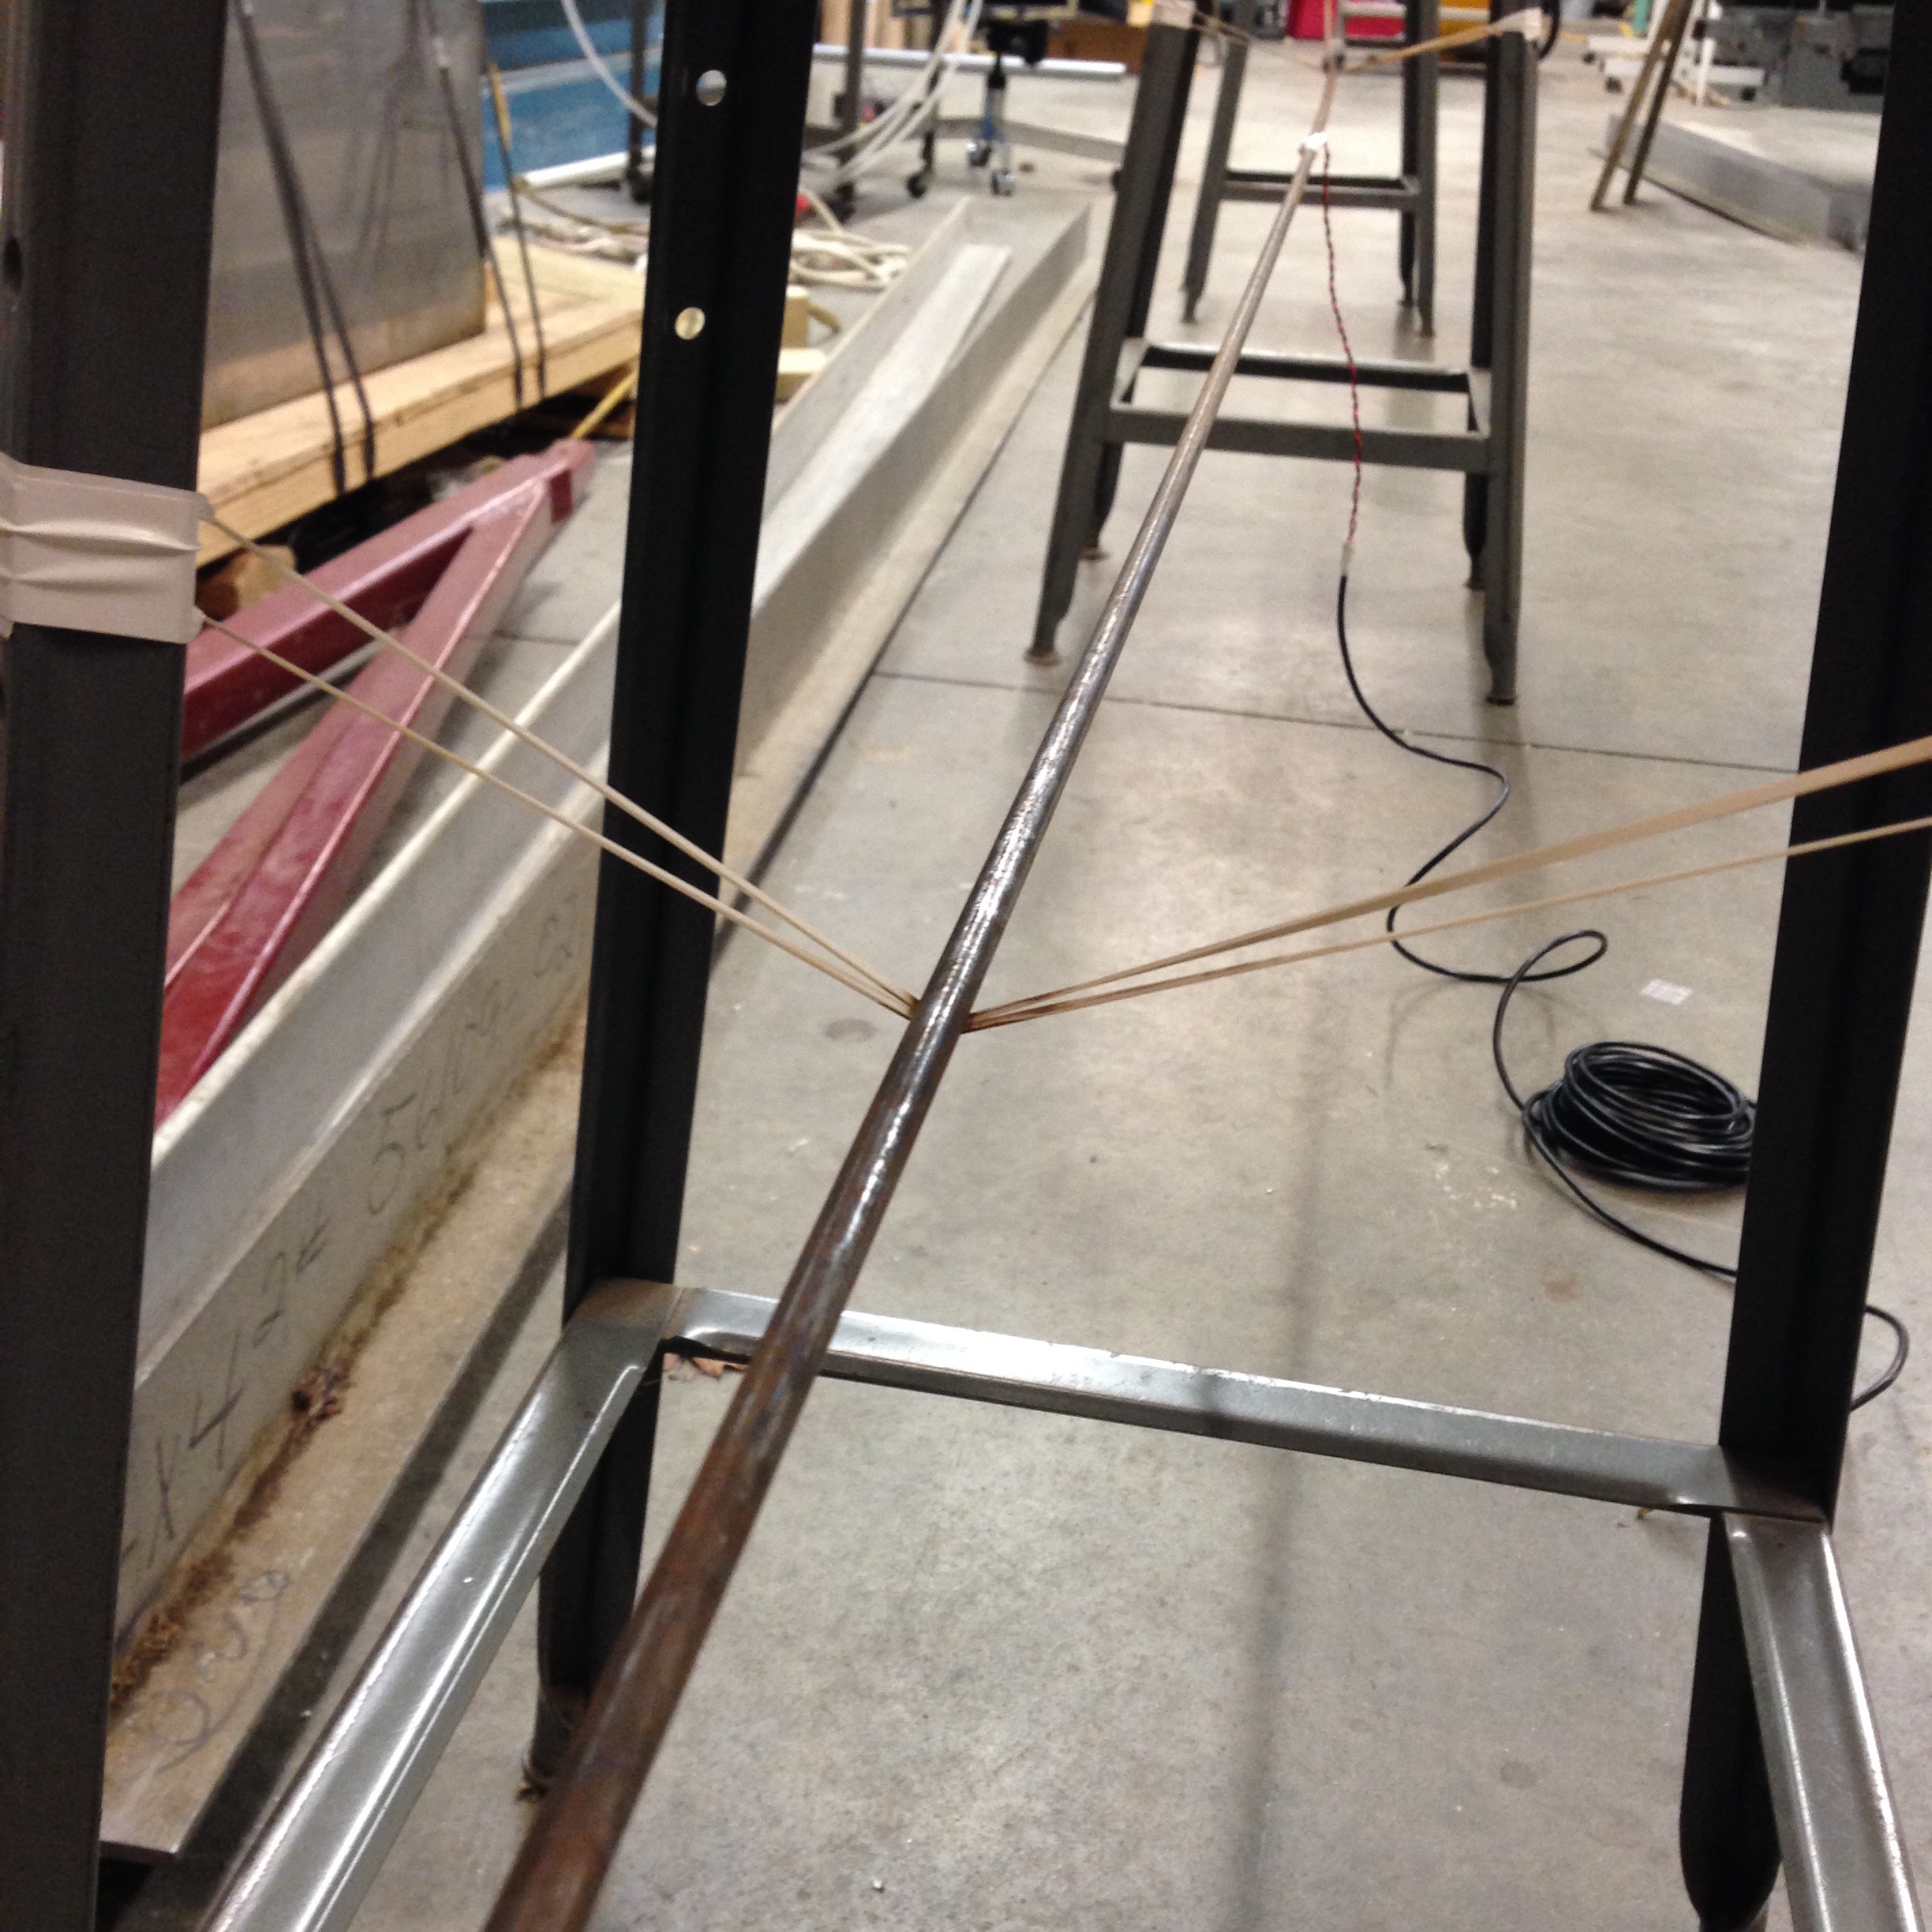
\includegraphics[width=.4\linewidth]{../figures/bands.jpg}
  \captionof{figure}{A figure}
  \label{fig:test1}
\end{minipage}%
\begin{minipage}{.5\textwidth}
  \centering
  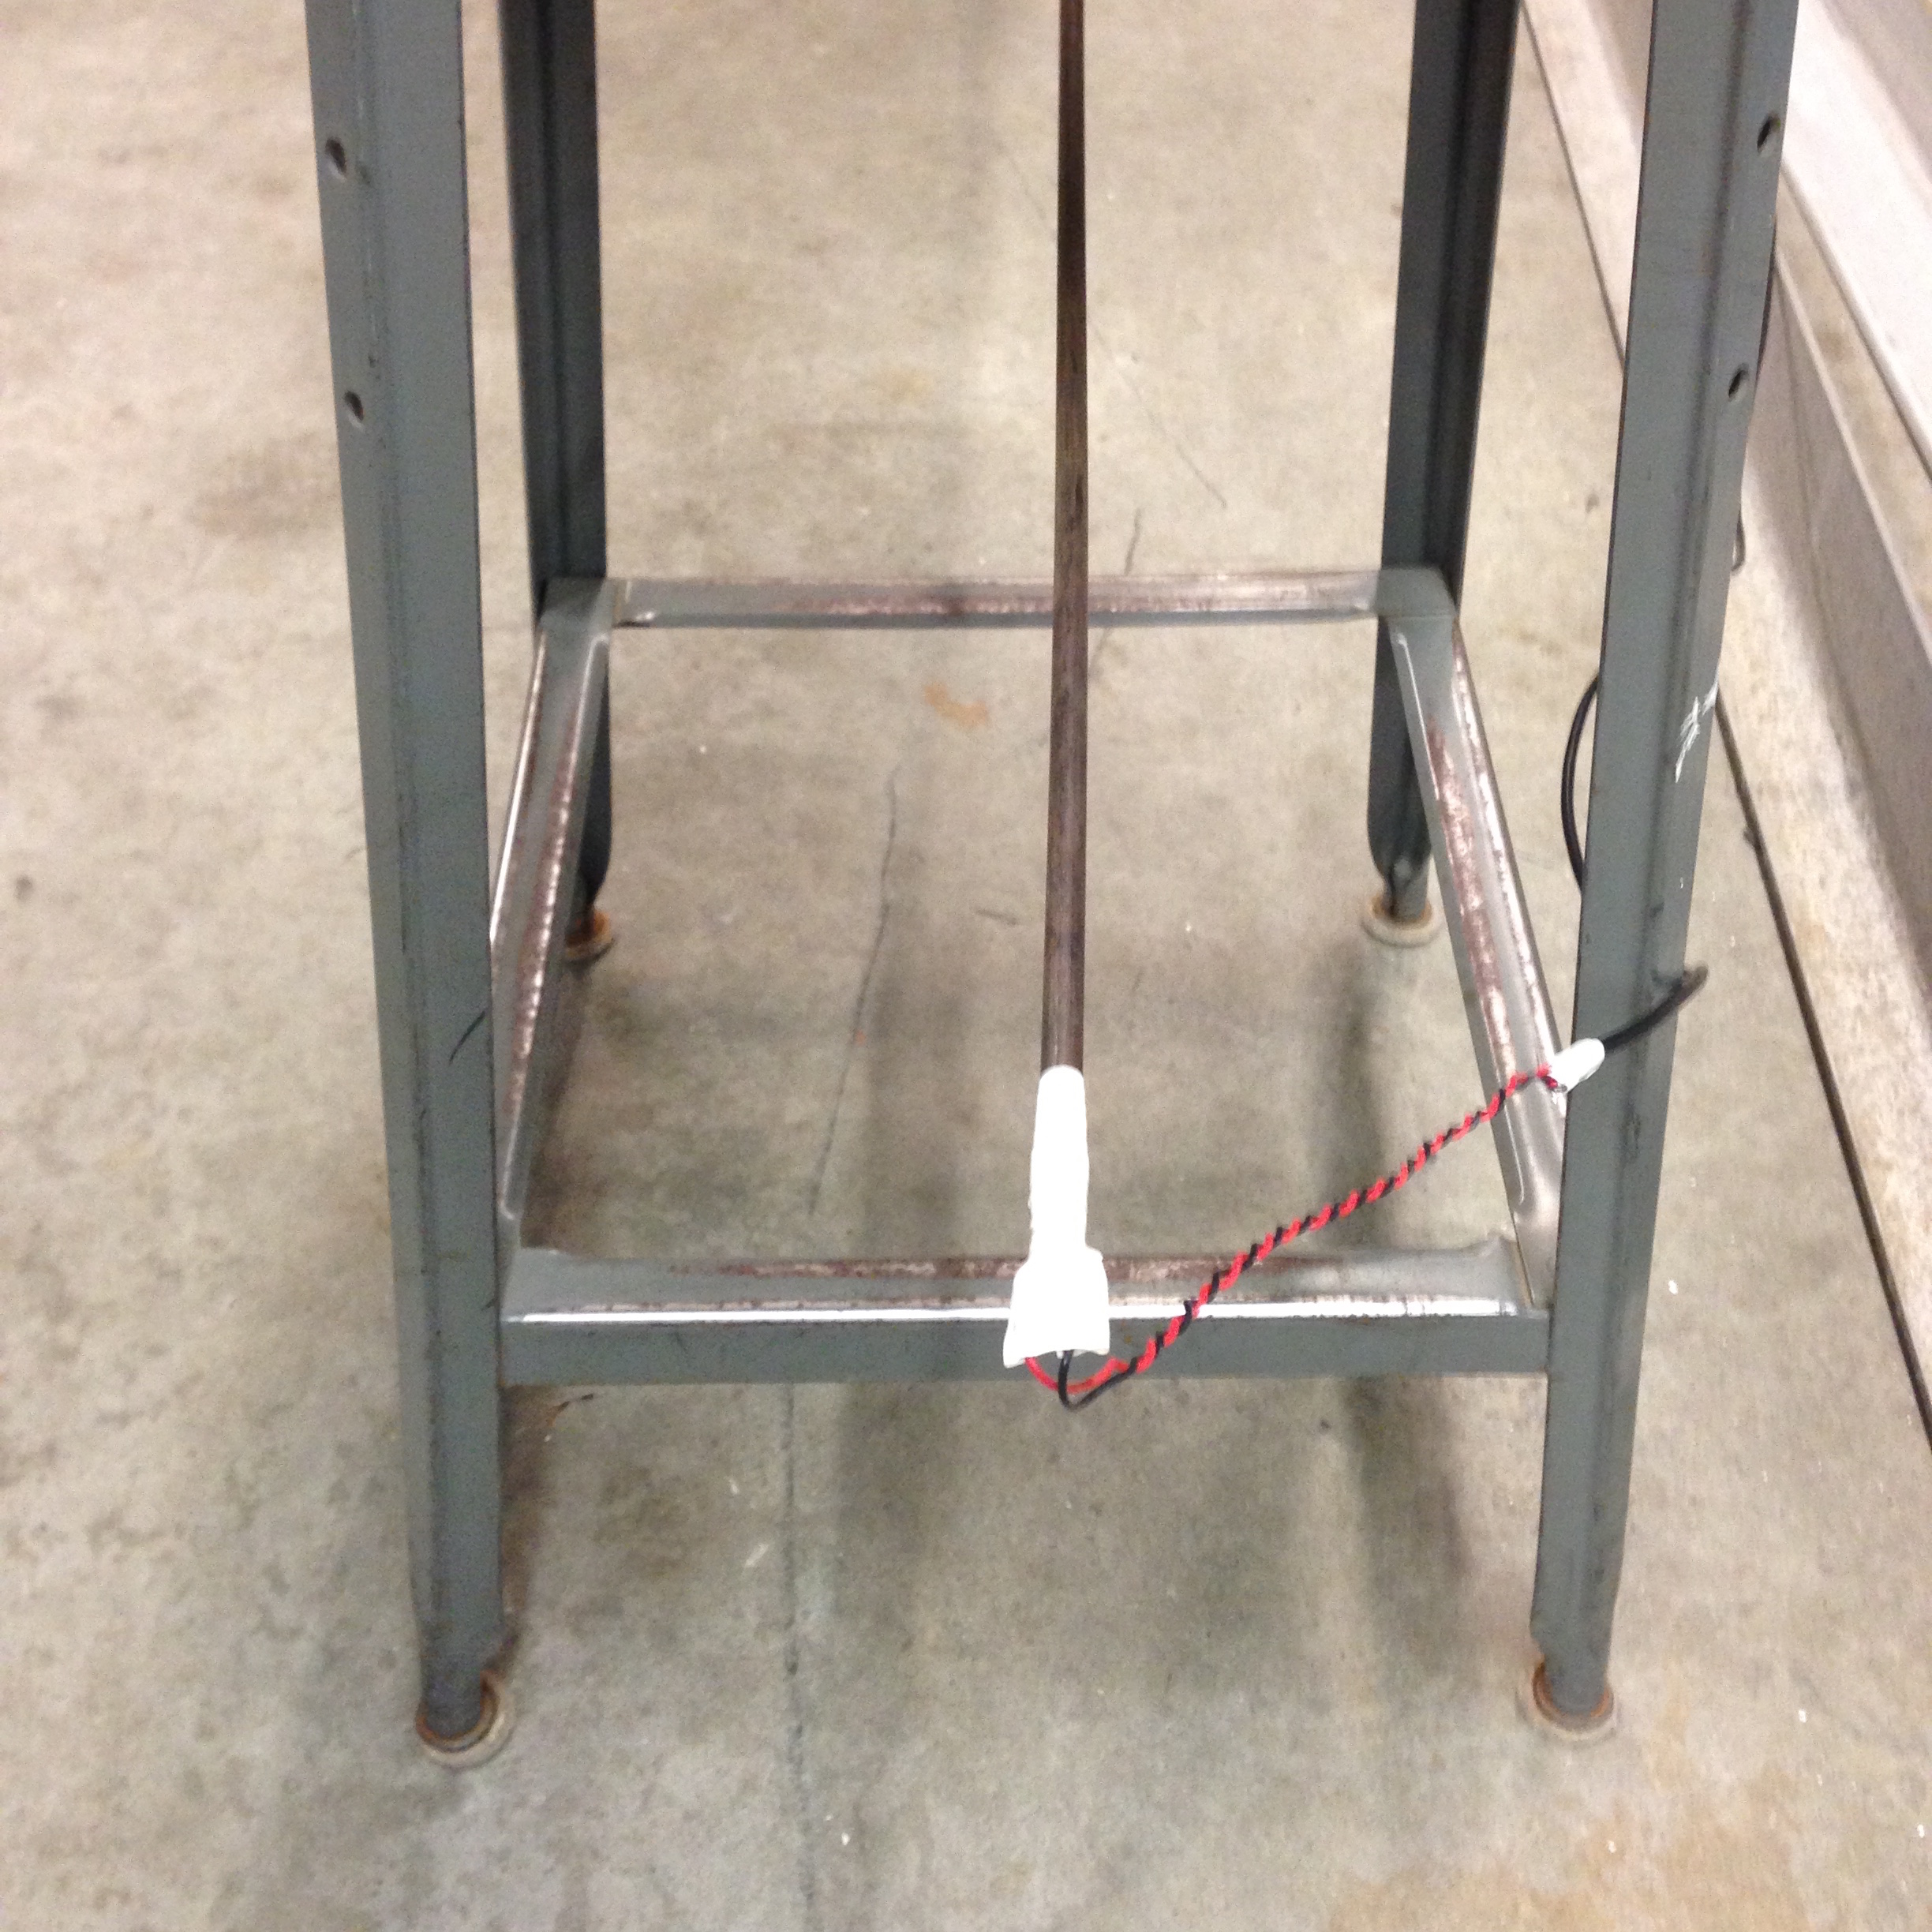
\includegraphics[width=.4\linewidth]{../figures/pmnt_end.jpg}
  \captionof{figure}{Another figure}
  \label{fig:test2}
\end{minipage}
\end{figure}
